\begin{figure*}[!h]
	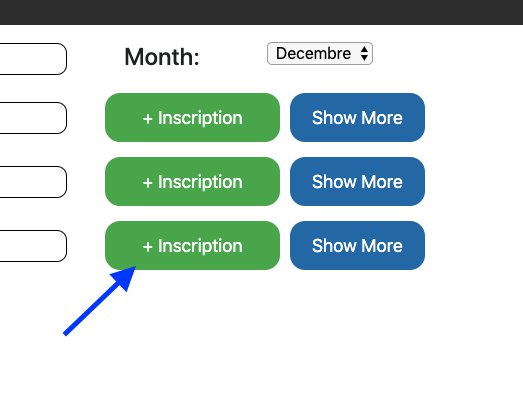
\includegraphics[width=0.5\textwidth,center]{Figures/us3-1}
	\caption{bouton d'inscritption}
\end{figure*}

\begin{enumerate}
	\item l'utilisateur choisit la session correspondant à sa demande.
	\item l'utilisateur clique sur le bouton  \textit{+ Inscription}
\end{enumerate}

\subsubsection{Gestion des erreurs}
	\begin{itemize}
		\item Si l'utilisateur ne possède plus d'abonnement, une erreur sera affichée lui signalant le problème. 
		\item Si la session est complète un message d'erreur sera affiché. 
	\end{itemize}
	
\subsubsection{Scripts concerné}
	\begin{itemize}
		\item \Href{https://github.com/victorsmits/Aquabike/blob/master/Symfony-Twig/src/Controller/MonthController.php}{MonthController.php}
		\item \Href{https://github.com/victorsmits/Aquabike/blob/master/Symfony-Twig/templates/month/month.html.twig}{month.html.twig}
		\item \Href{https://github.com/victorsmits/Aquabike/blob/master/Symfony-Twig/src/Entity/Session.php}{Session.php}
	\end{itemize}